\begin{figure}[!htb]
\begin{center}
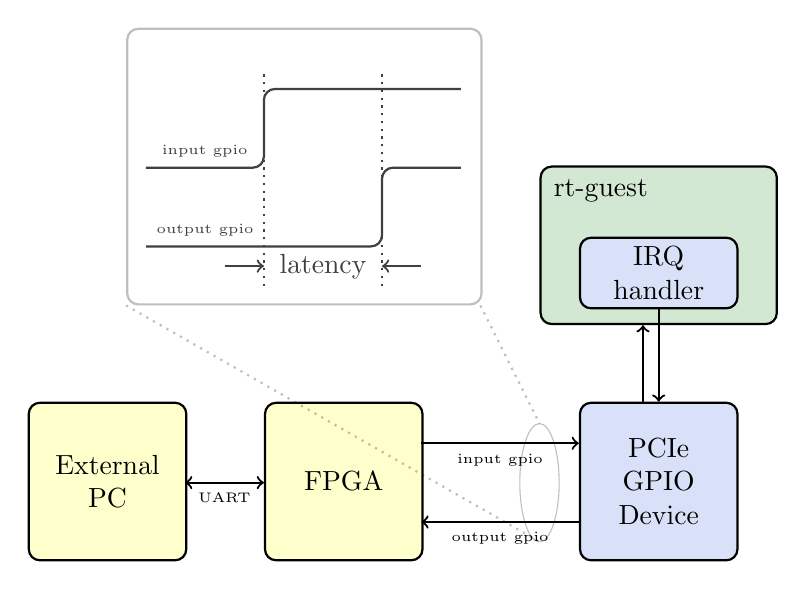
\begin{tikzpicture}

%\draw[step=1cm, gray, very thin, dotted] (0,0) grid (10,8);

\node at (0,0) [rectangle, draw=black, thick, fill=Yellow!20, rounded corners, minimum height = 2cm, minimum width = 2.0cm, align=center, text width=1.7cm, anchor=south west] (pc) 
		{External\\ PC};

\node at (3,0) [rectangle, draw=black, thick, fill=Yellow!20, rounded corners, minimum height = 2cm, minimum width = 2cm, anchor=south west] (fpga) 
		{FPGA};

\node at (7,0) [rectangle, draw=black, thick, fill=RoyalBlue!20, rounded corners, minimum height = 2cm, minimum width = 2cm, align=center, text width=1.7cm, anchor=south west] (pciedev) 
		{PCIe GPIO\\ Device};

\node at (6.5,3) [rectangle, draw=black, thick, fill=ForestGreen!20, rounded corners, minimum height = 2cm, minimum width = 3cm, align=center, text width=1.7cm, anchor=south west] (rtg) {};
\node[below right, inner sep=5pt] at (rtg.north west) {rt-guest};

\node at (7,3.2) [rectangle, draw=black, thick, fill=RoyalBlue!20, rounded corners, minimum height = 0.75cm, minimum width = 2cm, align=center, text width=1.7cm, anchor=south west] (irqhandler) 
		{IRQ handler};

\draw[black, thick, ->] (irqhandler.south) -- (pciedev);
\draw[black, thick, ->] ([xshift=-0.2cm]pciedev.north) -- ([xshift=-0.2cm]rtg.south) ;


\draw[black, thick, <->] (2,1) -- (3,1) node [below, midway, align=center] {\tiny{UART}};
\draw[black, thick, ->] (5,1.5) -- (7,1.5)  node [below, midway, align=center] {\tiny{input gpio}};
\draw[black, thick, <-] (5,0.5) -- (7,0.5)  node [below, midway, align=center] {\tiny{output gpio}};

\draw[black, rounded corners, thick] (1.5,5) -- (3,5) node [above, midway, align=center] {\tiny{input gpio}} -- (3,6) -- (5.5,6);
\draw[black, rounded corners, thick] (1.5,4) -- (4.5,4)  node [above left, midway, align=center] {\tiny{output gpio}} -- (4.5,5) -- (5.5,5);

\draw[black, thick, dotted] (3,3.5) -- (3,6.25);
\draw[black, thick, dotted] (4.5,3.5) -- (4.5,6.25);

\node (latency) at (3.75,3.75) [align=center, text width=1.5cm] {latency};
\draw[black, thick, ->] (2.5,3.75) -- (3,3.75);
\draw[black, thick, <-] (4.5,3.75) -- (5,3.75);

\begin {scope} [opacity=0.25]
\node at (1.25,3.25) [thick, rectangle, draw=black, thick, fill=white, rounded corners, minimum height = 3.5cm, minimum width = 4.5cm, anchor=south west] (lbox) {};
\draw [anchor=south west] {(6.5,1) ellipse (0.25cm and 0.75cm)};
\draw[black, thick, dotted] (1.25,3.25) -- (6.5,0.25);
\draw[black, thick, dotted] (5.75,3.25) -- (6.5,1.75);
\end {scope}


%\node at (1.25,3.25) [thick, ellipse, draw=black, thick, fill=white, rounded corners, minimum height = 1cm, minimum width = 0.5cm, anchor=south west] (gpios) {};

%\draw[black, thick, loosely dotted] (1.5,5) -- (3,5);

\end{tikzpicture}
\end{center}
\ifreport
\caption{Latency measurement setup}
\fi
\label{fig-measure-steup}
\end{figure}
